% !TEX root = master.tex

\chapter{Reduced Order Model}
\label{Ch:Deep Learning}
%\pagenumbering{arabic}



In this section model order reduction (ROM) will be introduced and two algorithms for obtaining a reduced basis (RB) are discussed. The proper orthogonal decomposition (POD) and autoencoders. In addition a reduced order model (ROM) based on the method of characteristics\cite{CFD1} is evaluated.\\
Model order reduction is a technique used for reducing the computational cost, which is computational resources as memory and computation power. Partial differential equations (PDEs) once discretized become a system of high dimensional ordinary differential equations (ODEs) as shown in \cref{Sec: BGK}. Here model order reduction exploits the idea that every high dimensional dynamical-state space\(f(\mathbf{x},\mathbf{\mu}) \in \mathcal{D}\)  can be described by a state-space or manifold of lower dimension \(\tilde{f}(\mathbf{\mu}) \in \mathcal{E}\)
\begin{equation}
	f \approx \tilde{f} \qquad\textrm{with}\qquad \mathcal{D} \ll \mathcal{E}.
\end{equation}
Reduced order modeling is partitioned into two successive phases called the \textit{offline} - and the \textit{online phase}. During the offline phase data or \textit{snapshots} of a dynamical-system is generated through experiments or simulations of the full order model (FOM). The so called \textit{snapshots} \(U = {u(t1),...,u(t_n)}\) are created once, each representing one moment in time of the dynamical system. Next a mapping \(g\) is constructed such that \(\tilde{u} = g(\tilde{u})\), for which \(u(t_i) \approx u(t_i)\). During the online phase the reduced order model is evaluated and the error is estimated by eg. \(||u(t) - \tilde{u}(t)\). Therefore the online phase may be described as stage of independence from the full order model. 
To continue the definition of the \textit{intrinsic solution manifold dimensionality} by \textit{Carlberg et al.} \cite{Carlberg} is needed: Assuming the initial value problem
\begin{equation}
	\mathbf{r}^n(\mathbf{x}^n;\mathbf{\mu}) = 0, \qquad n=1,...,N_t
\end{equation} 
has a unique solution for each parameter instance \(\mathbf{\mu} \in \mathcal{D}\), the intrinsic dimensionality of the solution manifold \(\{\mathbf{x}(t,\mathbf{\mu})|t \in [0,T],\mathbf
\mu \in \mathcal{D}\}\) is (at most) \(p^{\star} = n_{\mu} + 1\), as a mapping \((t,\mathbf{\mu})\mapsto \mathbf{x}\) is unique in this case. This provides a practical lower bound on the dimension of a nonlinear trial manifold for exactly representing the dynamical-system state. In summary the intrinsic solution manifold dimensionality, in the following referred to as the number of intrinsic variables, are in number as much as there are parameters that can describe the whole dynamical-system state plus one, the time \(t\). As for the full order BGK equation \cref{Sec: BGK} the intrinsic variables could be three for the macroscopic velocity \(U(\mathbf{x},t)\), three for the microscopic velocities \(\xi\)of the collision operator \(Q(f,f)\), three for \(T\),\(\rho\) and \(\nu\) plus one equaling to a total of ten intrinsic variables for the 3D case. In the following subsection the available data for this thesis is introduced along with a proposal for the number of intrinsinc variables.\\
The BGK equation is valid for gases in the hydrodynamic regime as well as for rarefied gases. As described in \cref{Sec: BGK} depending on the equilibrium of the BGK equation, the solution transitions between a pure Boltzmann - and a Maxwellian distribution. The former is known to be well approximated by linear methods as the SVD, while the latter poses problems due to the non-linear behavior.
\section{Offline Phase}
\subsection{Full order BGK model}\label{Sec: Data Sampling}
The number of intrinsic variables can therefore be determined for the 1D case of the BGK equation. The parameters \(\mathbf{\mu}\)describing the gas flow in the hydrodynamic regime has therefore one macroscopic velocity \(U(x)\), and th
DIE ORIGINAL DTATENSTRUJTUR BESCHREIBEN
For the autencoder using fully connected layers, the input vectors $y_o \in \mathbb{R}$ of size $n_{\text{input}} = n_{\xi} = 40$ are arranged in the sampling matrix $S_{AE} \in \mathbb{R}^{n_{\mathrm{S}\times n_\xi}}$ as seen in \cref{AE_matrix} resulting in $n_S = 5000$ available samples. Note that the POD uses the same matrix transposed $S_{AE}^T$ as input. In the following hydrodynamic regime will reffer for the input data for knudsen number 10e-4 and rarefied regime will refer to the input data for knudsen numbers 10e2.
- insert unshuffled set pls
\begin{multicols}{2}
	\begin{equation}
	S_{AE} = \begin{bmatrix}
	f(\xi_1,t_1,x_1)&\cdots &f(\xi_n,t_1,x_1) \\
	f(\xi_1,t_1,x_2)&\cdots &f(\xi_n,t_1,x_2) \\
	\vdots& \vdots & \vdots\\
	f(\xi_1,t_1,x_n)&\cdots &f(\xi_n,t_1,x_n)\\
	f(\xi_1,t_2,x_1)&\cdots &f(\xi_n,t_2,x_1)\\
	\vdots & \vdots & \vdots\\
	f(\xi_1,t_n,x_n)&\cdots &f(\xi_n,t_n,x_n)
	\end{bmatrix}
	\label{AE_matrix}
	\end{equation}\break
	\begin{equation}
	S_{Conv}= \begin{bmatrix}
	n_{Filters}&f(\xi_1,\textbf{t},\textbf{x})\\
	n_{Filters}&f(\xi_2,\textbf{t},\textbf{x})\\
	\vdots\\
	n_{Filters}&f(\xi_n,\textbf{t},\textbf{x})
	\end{bmatrix}
	\label{Conv_matrix}
	\end{equation}
\end{multicols}\noindent
Convolutional autoencoders use a different sampling matrix $S_{Conv}$ due to their two dimensional capability resulting in $n_S = 40$ available samples \cref{Conv_matrix}.$N_{Filters}$ varies over the succeeding layers, growing with the shrinkage of $(\textbf{t},\textbf{x})$.
- In the following the data of the BGK full order model with a knudens number of \(Kn = 0.00001\), describing a gasflow in the hyrodynamic regime will be reffere to as \(\Pi_h\). Equally the data of the BGK full order model with a knudsen number of \(Kn = 0.01\) will be refferd to as \(\Pi_r\).

\subsection{Reduced Basis by POD and Autoencoder}
The singular value decomposition of the input $X$ [REF to Section 1] gives the optimal low-rank approximation $\tilde{X}$ of $X$ \cref{Eg:eckard-young}[Eckard-Young].
\begin{equation}[!htbp]
\underset{\tilde{X}, s.t. rank(\tilde{X})=r}{\operatorname{argmin}} || X -\tilde{X} ||_F=\tilde{U}\tilde{\Sigma}\tilde{V}^*
\label{Eg:eckard-young}
\end{equation} 
\begin{figure}[!htbp]
	% This file was created by tikzplotlib v0.9.6.
\begin{tikzpicture}

\begin{groupplot}[group style={group size=2 by 1, horizontal sep=1cm, vertical sep=2cm}]
\nextgroupplot[
log basis y={10},
tick align=outside,
tick pos=left,
x grid style={white!69.0196078431373!black},
xlabel={\(k\)},
xmin=-0.95, xmax=41.95,,
xtick style={color=black},
y grid style={white!69.0196078431373!black},
ylabel={\(\sigma\)},
ymin=2.86160392849359e-16, ymax=240.32740800328,
ymode=log,
ytick style={color=black},
ytick={1e1,1e-3,1e-11,1e-15},
width=.55\textwidth,
height=.7\textwidth,
y label style={yshift=-2.5em},
grid=both
]
\addplot [semithick, red, mark=o, mark size=2, mark options={solid}]
table {%
1 36.8185958349281
2 5.78483852846218
3 2.9488881352441
4 1.08115123432794
5 0.4715894924307
6 0.27551553286601
7 0.155493855631619
8 0.0601331453526982
9 0.05155511017701
10 0.0132542951500055
11 0.0118122790965581
12 0.00208495452053553
13 0.00184461993287337
14 0.000261109297076443
15 0.000174118703867616
16 2.59262125849959e-05
17 1.30752219185821e-05
18 1.92140998809572e-06
19 9.1685066176197e-07
20 1.08651788755093e-07
21 5.26354986735524e-08
22 4.52124036969183e-09
23 2.44729256168519e-09
24 1.43747068296607e-10
25 9.28350136149776e-11
26 3.39879764456285e-12
27 2.74182349854538e-12
28 6.4789443879917e-14
29 6.12293316992491e-14
30 1.6313694307166e-14
31 2.92181471455653e-15
32 2.92181471455653e-15
33 2.92181471455653e-15
34 2.92181471455653e-15
35 2.92181471455653e-15
36 2.92181471455653e-15
37 2.92181471455653e-15
38 2.92181471455653e-15
39 2.92181471455653e-15
40 1.8678655154319e-15
};

\nextgroupplot[
tick align=outside,
tick pos=left,
x grid style={white!69.0196078431373!black},
xlabel={\(k\)},
xmin=-0.95, xmax=41.95,
xtick style={color=black},
y grid style={white!69.0196078431373!black},
ylabel={cusum-e},
ymin=0.760859233580134, ymax=1.0113876555438,
ytick style={color=black},
ytick={1,.8},
width=.55\textwidth,
height=.7\textwidth,
y label style={yshift=-2em},
grid=both
]
\addplot [semithick, red, mark=o, mark size=2, mark options={solid}]
table {%
1 0.772246889123937
2 0.893580238655189
3 0.95543131247198
4 0.978107779579132
5 0.987999072557982
6 0.993777837563443
7 0.997039223381299
8 0.998300478281949
9 0.999381814290284
10 0.999659814794242
11 0.999907569918492
12 0.999951300528145
13 0.99998999027099
14 0.999995466874262
15 0.999999118904556
16 0.999999662690558
17 0.999999936935114
18 0.99999997723548
19 0.999999996465846
20 0.999999998744749
21 0.999999999848745
22 0.999999999943575
23 0.999999999994906
24 0.999999999997921
25 0.999999999999868
26 0.999999999999939
27 0.999999999999997
28 0.999999999999998
29 0.999999999999999
30 1
31 1
32 1
33 1
34 1
35 1
36 1
37 1
38 1
39 1
40 1
};
\addplot [thick, , mark=x,black, mark size=2, mark options={solid}]
table{%
6 0
6 0.993777837563443
6 1.3
};
\end{groupplot}
\end{tikzpicture}


	\label{Fig:CumSum_Rare}
	\caption{Sigular values \(\sigma\) over \(k\) number of singular values left and \(cumultative\) \(energy\) over \(k\) right for the gas flow in the rarefied regime.}
\end{figure}
\begin{figure}[!htbp]
	% This file was created by tikzplotlib v0.9.6.
\begin{tikzpicture}

\begin{groupplot}[group style={group size=2 by 1, horizontal sep=1cm, vertical sep=2cm}]
\nextgroupplot[
log basis y={10},
tick align=outside,
tick pos=left,
x grid style={white!69.0196078431373!black},
xlabel={\(k\)},
xmin=-0.95, xmax=41.95,,
xtick style={color=black},
y grid style={white!69.0196078431373!black},
ylabel={\(\sigma\)},
ymin=2.86160392849359e-16, ymax=240.32740800328,
ymode=log,
ytick style={color=black},
ytick={1e1,1e-3,1e-11,1e-15},
width=.55\textwidth,
height=.7\textwidth,
y label style={yshift=-2.5em},
grid=both
]
\addplot [semithick, red, mark=o, mark size=2, mark options={solid}]
table {%
1 36.8185958349281
2 5.78483852846218
3 2.9488881352441
4 1.08115123432794
5 0.4715894924307
6 0.27551553286601
7 0.155493855631619
8 0.0601331453526982
9 0.05155511017701
10 0.0132542951500055
11 0.0118122790965581
12 0.00208495452053553
13 0.00184461993287337
14 0.000261109297076443
15 0.000174118703867616
16 2.59262125849959e-05
17 1.30752219185821e-05
18 1.92140998809572e-06
19 9.1685066176197e-07
20 1.08651788755093e-07
21 5.26354986735524e-08
22 4.52124036969183e-09
23 2.44729256168519e-09
24 1.43747068296607e-10
25 9.28350136149776e-11
26 3.39879764456285e-12
27 2.74182349854538e-12
28 6.4789443879917e-14
29 6.12293316992491e-14
30 1.6313694307166e-14
31 2.92181471455653e-15
32 2.92181471455653e-15
33 2.92181471455653e-15
34 2.92181471455653e-15
35 2.92181471455653e-15
36 2.92181471455653e-15
37 2.92181471455653e-15
38 2.92181471455653e-15
39 2.92181471455653e-15
40 1.8678655154319e-15
};

\nextgroupplot[
tick align=outside,
tick pos=left,
x grid style={white!69.0196078431373!black},
xlabel={\(k\)},
xmin=-0.95, xmax=41.95,
xtick style={color=black},
y grid style={white!69.0196078431373!black},
ylabel={cusum-e},
ymin=0.760859233580134, ymax=1.0113876555438,
ytick style={color=black},
ytick={1,.8},
width=.55\textwidth,
height=.7\textwidth,
y label style={yshift=-2em},
grid=both
]
\addplot [semithick, red, mark=o, mark size=2, mark options={solid}]
table {%
1 0.772246889123937
2 0.893580238655189
3 0.95543131247198
4 0.978107779579132
5 0.987999072557982
6 0.993777837563443
7 0.997039223381299
8 0.998300478281949
9 0.999381814290284
10 0.999659814794242
11 0.999907569918492
12 0.999951300528145
13 0.99998999027099
14 0.999995466874262
15 0.999999118904556
16 0.999999662690558
17 0.999999936935114
18 0.99999997723548
19 0.999999996465846
20 0.999999998744749
21 0.999999999848745
22 0.999999999943575
23 0.999999999994906
24 0.999999999997921
25 0.999999999999868
26 0.999999999999939
27 0.999999999999997
28 0.999999999999998
29 0.999999999999999
30 1
31 1
32 1
33 1
34 1
35 1
36 1
37 1
38 1
39 1
40 1
};
\addplot [thick, , mark=x,black, mark size=2, mark options={solid}]
table{%
6 0
6 0.993777837563443
6 1.3
};
\end{groupplot}
\end{tikzpicture}


	\label{Fig:CumSum_Hydro}
	\caption{Sigular values \(\sigma\) over \(k\) number of singular values left and \(cumultative\) \(energy\) over \(k\) right for the gas flow in the hydrodynamic regime.}
\end{figure}
\begin{table}[!htbp]\centering
\begin{tabular}{ |c|c|c|c|c|c|c|c|c| }
	\hline
	Intrinsic variables  & 3 & 4 & 5 & 6 & 7 & 8 & 9 & 10 \\ %[.5ex]
	\hline
	Error & 0.0327 & 0.0153 & 0.0087 & 0.0046 & 0.0021 & 0.0014 & 0.0005 & 0.0003\\ \hline
\end{tabular}
\caption{L2-Error for different numbers of intrinsic variables for the rarefied gas flow. Calculations with two intrinsic variables are also performed, but not shown here because two intrinsic variables is considered trivial.}
\label{Tab:Intrinsic units svd rare}
\end{table}
\begin{table}[!htbp]\centering
	\begin{tabular}{ |c|c|c|c|c|c|c|c|c| }
		\hline
		Intrinsic variables  & 3 & 4 & 5 & 6 & 7 & 8 & 9 & 10 \\ %[.5ex]
		\hline
		Error & 0.0205 & 0.0081 & 0.0030 & 0.0013 & 0.0006 & 0.0002 & 6.2\(e^{-5}\) & 2.7\(e^{-5}\)\\ \hline
	\end{tabular}
	\caption{L2-Error for different numbers of intrinsic variables for the hydrodynamic gas flow. Calculations with two intrinsic variables are also performed, but not shown here because two intrinsic variables is considered trivial.}
	\label{Tab:Intrinsic units svd hydro}
\end{table}
\textbf{}\subsection{Online Phase}
loremipsu
\subsection{Reduced Order Model}\label{Reduced Order Model}
The compression of the input data $y_0$ yields a code $C \in \mathbb{R}^{ix5000}$, composed  of the instrinsic variables \(c_i\). The index \(i\) corresponds to the i-th intrinsic variable whereas their number is given by the input data. Each of them describes the transport of a discontinuity as seen in \cref{Fig:Code_Fully}. Hence the expolitability of the code in terms of constructing a ROM is not provided. On that account the method of characteristics \cite{Dret2016} provides a means to bypass this shortage. It is necessary for $c_i(x,t)$ to satisfy the conservative condition \cref{Eq. Mass_Const} and the transport equation \cref{Eq. Transport}.\\
\noindent\begin{minipage}{.5\linewidth}
	\begin{equation}
	\frac{d}{dt}\int c_i\ dx = \frac{d}{dt}f_i = const. \label{Eq. Mass_Const}
	\end{equation}
\end{minipage}%
\begin{minipage}{.5\linewidth}
	\begin{equation}
	\frac{\partial}{\partial t}c_i + \frac{\partial}{\partial x}f_i = 0 \label{Eq. Transport}
	\end{equation}
\end{minipage}
The characteristics $u_i$ describe the constant transport velocities for each variable $c_i$ calculated using \cref{Eq. Characteristics}. Subsequently enabling the usage of a simple plynomial interpoaltion of any degree. Furthermore a linear mapping \(A_ix_i=c_i\) can be applied for the reconstruction of interpolated code variables \(\hat{c}_i\). \Cref{Fig. Flowchart} depicts this approach in detail.\\
Questions concering the capacity of this ROM, e.g. how many samples \(\hat{n}_t\) are needed to reconstruct \(n_t\) timestamps, are analysed in \cref{Results}.
\begin{equation}
	u_i = \frac{f_i(c^-_i) - f_i(c^+_i)}{c^-_i - c^+_i}
	\label{Eq. Characteristics}
\end{equation}
\begin{figure}
	\centering
	\usetikzlibrary{matrix}
\usetikzlibrary{shapes,snakes}
	\tikzstyle{rec} = [rectangle, rounded corners, minimum width=1cm, minimum height=1cm,text centered, draw=black]
	\tikzstyle{circ} = [circle,minimum size =1.5cm,text centered, draw=black]
	\tikzstyle{arrow} = [thick,->,>=stealth]
		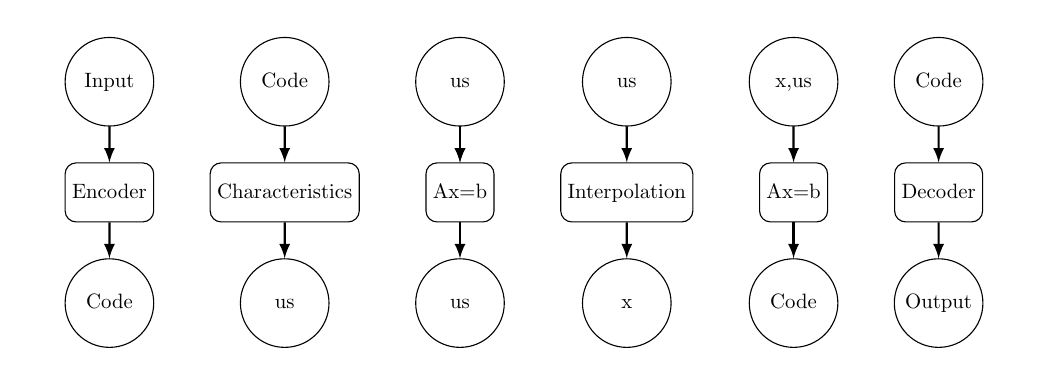
\begin{tikzpicture}[>=latex,text height=1.5ex,text depth=0.25ex,scale=.5,every node/.style={scale=0.75}]
		\matrix[matrix of nodes,column sep= 1em,row sep= 3ex]{
			&
			\node[circ] (1) {Input};&
			&
			\node[circ] (4) {Code};&
			&
			\node[circ] (7) {us};&
			&
			\node[circ] (10) {us};&
			&
			\node[circ] (13) {x,us};&
			&
			\node[circ] (16) {Code};&
			\\
			&
			\node[rec] (2) {Encoder};&
			&
			\node[rec] (5) {Characteristics};&
			&
			\node[rec] (8) {Ax=b};&
			&
			\node[rec] (11) {Interpolation};&
			&
			\node[rec] (14) {Ax=b};&
			&
			\node[rec] (17) {Decoder};&
			\\
			&
			\node[circ] (3) {Code};&
			&
			\node[circ] (6) {us};&
			&
			\node[circ] (9) {us};&
			&
			\node[circ] (12) {x};&
			&
			\node[circ] (15) {Code};&
			&
			\node[circ] (18) {Output};&
			\\
		};
	\path[->]
		(1) edge[thick] (2)
		(2) edge[thick] (3)
		(4) edge[thick] (5)
		(5) edge[thick] (6)
		(7) edge[thick] (8)
		(7) edge[thick] (8)
		(8) edge[thick] (9)
		(10) edge[thick] (11)
		(11) edge[thick] (12)
		(13) edge[thick] (14)
		(14) edge[thick] (15)
		(16) edge[thick] (17)
		(17) edge[thick] (18);
\end{tikzpicture}
	\caption{This figure shows the steps for obtaining a reduced oder model (ROM). Decoder and Encoder need to be used after training. In step one $y_0$ is the original input data, $C$ is the Code. In step two $c_i$ is the i-th intrinsic variable and $u_i$ the correspnding characteristic. The eigenvalue problem in step 3 outputs $x_i$ the eigenvector of A, a diagonal matrix composed of $u_i$ and b is the corresponing i-th intrinsic variable $c_i$. In step 4 $\hat{u}_i$ is the interpolated vector to $u_i$. Step 5 solves the linear equation for the diagonal matrix A composed of $\hat{u}_i$ times the eigenvector $x_i$ of the eigenvalueproblem in step 3. The output is $\hat{c}_i$ the i-th intrinsic variable corresponding to $\hat{u}_i$ the i-th interpolated characteristic.}
	\label{Fig. Flowchart}
\end{figure}